% capnocolon用于去掉图表标题中的冒号;
% titleahuart为AHU文科的章节标题格式,
% 理科请将titileahuart改为titleahuscience,
% 若要使用USTC格式请改为titlechinese;
% oneside, openany为单面选项,
% 若要双面且章节从奇数页开始,
% 请改为twoside, opentight;
\documentclass[capnocolon,titleahuscience,oneside,openany]{ahuthesis}
\usepackage{metalogo}
\usepackage{verbatim}
\usepackage{titlesec}
\usepackage{unicode-math}
%\renewcommand\thesection{\arabic {section}}
% 设置图形文件的搜索路径
\graphicspath{{chapter/}{figure/}}
%=================设置章节标题格式==================
\ctexset{
	section={
		%format用于设置章节标题全局格式,作用域为标题和编号
		%字号为小三,字体为黑体,左对齐
		%+号表示在原有格式下附加格式命令
		format+ =\heiti
	},
	subsection={
		%format用于设置章节标题全局格式,作用域为标题和编号
		%字号为小三,字体为黑体,左对齐
		%+号表示在原有格式下附加格式命令
		format+ =\heiti
	},
}

\begin{document}
%%%%%%%%%%%%%%%%%%%%%%%%%%%%%%
%% 封面部分
%%%%%%%%%%%%%%%%%%%%%%%%%%%%%%
% 封面内容
% 当中文标题过长时可以将多余的标题放在\titletail{}中
\title{模糊最大熵聚类模型及其应用}
\entitle{Fuzzy Maximum Entropy Clustering Model and Its Application}
%全角空格可以正常输出
\author{覃浩蓝}
\enauthor{Qin Hao Lan }
\department{数学科学学院}
\No{A01714003}
\tutor{吴 涛}
\entutor{Prof. Wu Tao}
\cntime{二〇二一年五月}
\entime{May,2021}
\major{信息与计算科学}
\enrolltime{二〇一七年 九月}
\tutordegree{教授/博士}
\tutordepartment{数学科学学院}

% 生成USTC格式的中英文合并的扉页,AHU可以使用
%\maketitle

%生成安徽大学格式的扉页
\makeahutitle

%%%%%%%%%%%%%%%%%%%%%%%%%%%%%%
%% 前言部分
%%%%%%%%%%%%%%%%%%%%RN1%%%%%%%%%%
\frontmatter

% 题目、摘要、关键词
\begin{cnabstract}
  在模糊C均值(Fuzzy C-means)算法中,通过与模糊数学的融合,给出了相比于K-means硬聚类更灵活的聚类结果。
  \cnkeywords{模糊熵,最大熵,聚类}
\end{cnabstract}

\begin{abstract}
  In the.
  \par
  \keywords{Fuzzy Sets;}
\end{abstract} 
% 目录
\tableofcontents

%%%%%%%%%%%%%%%%%%%%%%%%%%%%%%
%% 正文部分
%%%%%%%%%%%%%%%%%%%%%%%%%%%%%%
\mainmatter
\chapter[绪论]{绪论}
%\section{绪论}
\section{研究背景}
\par
进入信息时代后,我们对信息的获取和加工能力在不断进步,我们周围的信息越来越多,五花八门各式各样的信息充斥在我们的生活中,这些信息有的是确定的,但更多的是不确定的、带有模糊性的信息.
所谓模糊性是指不确定的,介于是和不是两者之间的性质.
例如,对于优等生的判定,有的人觉得90就可以了,有的人却觉得需要达到95分以上才算优秀,所以我们很难这种非此即彼的性质去衡量一个人是不是优等生.
\par
我们所处的是一个复杂多变、时刻在运动的世界,大到星系运动,小到粒子碰撞,里面蕴含的规律都是复杂多样的.
信息本身就包含着确定性和不确定性,无所谓的好坏之分,它取决于我们如何认识信息,了解信息和使用信息.
比如,我们在评价某一个菜品时,会用“好吃”、“还行“、”难吃“来形容;描述天气时说“多云”、 “晴朗”;说一个人的衣服搭配好看等等.
这些问题很难用统一的标准去衡量,但是我们已经习惯在生活中运用模糊性所谓语言描述事物,用模糊的方法认识生活中的事物.
虽然信息带着不确定性,但是我们所处的客观世界是确定的,所以我们需要一种方法研究模糊的信息,得到清晰的结论.于是数学诞生了一个新的分支:模糊数学.
\par
1965年,L.A.Zadeh在期刊Information and Control上发表了论文《Fuzzy Sets》\cite{ZADEH1965fuzzy},标志着模糊理论的诞生.
随后,1968年,L.A.Zadeh又发表了《Probability Measures of Fuzzy Events》\cite{zadeh1968probability},进一步补充模糊理论框架.
此后模糊理论开始进入广大学者的视野,不断得到完善和改进,并在控制理论领域得到广泛应用.
\section{研究内容}
最大熵模型是一种分类学习模型,模糊熵是模糊数学里面的概念,本文在模糊理论框架下,将最大熵推广到模型信息情形,在传统的模糊C均值聚类(FCM)上进行改进,建立模糊最大熵模型并应用于实际的分类问题中,通过进一步的研究 探索模糊最大熵模型在实际问题中的应用.
\section{研究意义}
随着人工智能的大热,机器学习开始迅速应用于我们的生活中,比如商品推荐、语音识别和智能导航等.
其中,分类问题是机器学习领域的一个重要问题.
生活中许多的分类问题是模糊的,计算机无法直接处理这些模糊信息,而我们的人脑却可以很好地从这些模糊信息中得到精确的结论.
随着熵理论和模糊数学的发展,模糊数学和最大熵模型的应用范围也越来越广泛,为了处理分类问题中的不确定性,国内外的许多这方面的学者也进行了许多研究,寻找分类问题模糊性的度量方式,探寻新的实际应用.本文将模糊熵与最大熵原理结合,
%TEX root=../main.tex
\chapter[预备知识]{预备知识}
聚类方法不仅是揭示给定数据集的基本结构的主要工具,也是揭示复杂系统的局部输入-输出关系的有效工具.
这自然引起了许多学者的兴趣,并由此产生了许多的聚类方法,模糊聚类就是其中一种.
正如我们所知道的, 聚类问题是一个优化问题:一组物体被分割成一个合理的 具有某些特征的子群.
这往往是在主观选择的测量函数的基础上,将一组物体分成合理数量的子组,使子组内物体之间的距离小于属于不同子组的物体之间的距离.
对现有的聚类方法进行改进是一个非常困难的问题,在这之前我们先了解一下模糊C-均值算法(FCM)方法.
\section{模糊集及其表示方法}
\par
在经典集合理论里面,一个集合就是某一个概念的内涵.
对于论域上的一个对象,它要么属于这个集合,要么不属于这个集合,两者只能选一个,不能两者兼之,也不能有模棱两可的情况.
而对模糊数学研究的对象来说,我们不能简单地用是或否来描述一个对象是否属于一个集合.
由此,我们把集合的特征函数的取值从$\{0,1\}$这个集合扩充到$[0,1]$这个区间上的连续取值.
越靠近1,说明该对象属于集合的程度越大,反之,越靠近0就越小.
%概括地说,模糊数学就是将现实世界的模糊概念抽象出来作为研究对象,然后用精确的数学方法探寻其中的数量规律的一门数学分支.
这样我们就把经典集合扩充到带有模糊边界的模糊集了,从而我们可以用这样的集合表示模糊概念.
\subsection{模糊集的定义}
\begin{definition}[模糊子集\scite{ZADEH1965fuzzy}]
    设$\mathrm{U}$为我们所研究的论域,
    \[
        \mu_{\tilde{A}}: \mathrm{U} \longrightarrow[0,1]
    \]
    称$\mu$确定了$\mathrm{U}$上的一个模糊子集,记为$\tilde{A}$.
    $\mu$称为$\tilde{A}$的隶属函数,把$\mu_{\tilde{A}}(u)(u \in \mathrm{U})$的值称为$u$对于模糊子集$\tilde{A}$的隶属度.
    $\mu_{\tilde{A}}(u)$越大,代表$u$隶属于$\tilde{A}$的程度越高.
    通常,我们也把模糊子集简称为模糊集.
\end{definition}
\subsection{模糊集的表示方法}
设有限集$\mathrm{U}=\{u_1,u_2,\dots ,u_n\}$,则有限集可以用如下几种方法表示\cite{模糊数学李安贵}.
\begin{itemize}
    \item Zadeh表示法
          \[
              \tilde{A}=\frac{\tilde{A}(u_1)}{u_1}+\frac{\tilde{A}(u_2)}{u_2}+ \dots +\frac{\tilde{A}(u_n)}{u_n}.
          \]
          虽然我们以分式和的方式表示,但是其中的$\tilde{A}(u_i)/u_i$并不表示分数,“+”也不表示和.
          $\tilde{A}(u_i)/u_i$表示的是元素$u_i$与对$\tilde{A}$的隶属度的一一对应关系;“+”表示的是$\tilde{A}$在论域$\mathrm{U}$上的整体.\newpage
    \item 序偶表示法
          \[
              \tilde{A}=\{(\tilde{A}(u_1),u_1),(\tilde{A}(u_2),u_2),\dots ,(\tilde{A}(u_n),u_n)\}.
          \]
          序偶表示法是从例举法演变而来,由元素的隶属度和对应的元素组成的有序对列出.
    \item 向量表示法
          \[
              \tilde{A}=(\tilde{A}(u_1),\tilde{A}(u_2),\dots ,\tilde{A}(u_n)).
          \]
          向量表示法是用n维数组来实现的,在论域中的元素按一定的顺序排列时,按此顺序记录元素的隶属度.
          此时也称$\tilde{A}$为模糊向量.
\end{itemize}
\section{模糊集的运算及其性质}
我们先给出模糊幂集的定义:
\begin{definition}
    论域$\mathrm{U}$上的模糊子集的全体称为模糊幂集,记为$\mathscr{F}(U)$,即
    \[
        \mathscr{F}(U)=\{\tilde{A} \mid \tilde{A}(u):\mathrm{U} \to [0,1]\}
    \]
\end{definition}
模糊集的包含与相等:
\begin{definition}
    设$\tilde{A}, \tilde{B} \in \mathscr{F}(U)$,如果对$\forall u \in \mathrm{U}$
    都成立$\tilde{B}(u)\geqslant \tilde{A}(u)$,则称$\tilde{B}$包含$\tilde{A}(u)$,记作$\tilde{B}(u )\supseteq \tilde{A}(u)$.
\end{definition}
\begin{definition}
    设$\tilde{A}, \tilde{B} \in \mathscr{F}(U)$,如果对$\forall u \in \mathrm{U}$
    都成立$\tilde{B}(u) = \tilde{A}(u)$,则称$\tilde{B}$等于$\tilde{A}(u)$,记作$\tilde{B}(u)= \tilde{A}(u)$.
\end{definition}
我们规定$a\vee b=MAX(a,b),a\wedge b=MIN(a,b)$,所以我们可以这样描述模糊集的并、交、余:

\begin{definition}
    如果对于任意一个$u \in \mathrm{U}$,有$\tilde{C}(u)=\tilde{A}(u) \vee \tilde{B}$,
    则称$\tilde{C}$为$\tilde{A}$与$\tilde{B}(u)$的并,记为$\tilde{C}=\tilde{A} \cup \tilde{B}$.
    如果对于任意一个$u \in \mathrm{U}$,有$\tilde{C}(u)=\tilde{A}(u) \wedge \tilde{B}$,
    则称$\tilde{C}$为$\tilde{A}$与$\tilde{B}(u)$的交,记为$\tilde{C}=\tilde{A} \cap \tilde{B}$.\\
    它们的隶属度函数定义为:
    \[
        (\tilde{A}\cup  \tilde{B})(u) \stackrel{\text { def }}{=}\tilde{A}(u) \vee \tilde{B}(u) , \forall u \in \mathrm{U}
    \]
    \[
        (\tilde{A}\cap   \tilde{B})(u) \stackrel{\text { def }}{=}\tilde{A}(u) \wedge \tilde{B}(u) ,\forall u \in \mathrm{U}
    \]
\end{definition}
\begin{definition}
    如果对于$\forall u \in \mathrm{U}$,有$\tilde{B}(u)=1-\tilde{A}(u) $,
    则称$\tilde{B}$为$\tilde{A}$的余,记为$\tilde{B}=\tilde{A}^c$.
\end{definition}
\section{模糊C-均值算法}
C-均值聚类是我们聚类经常用的方法之一,通过迭代计算使得目标函数达到局部最小值的时候,就是我们的最优分类.
在模糊C-均值聚类中,我们定义目标函数为:
\begin{equation}
    J(A, V)=\sum_{i=1}^{c} \sum_{j=1}^{n}\left(a_{i j}\right)^{r} d_{i j}^2
\end{equation}
$U=\{u_1,u_2,\dots,u_n\},u_j=(x_{j1},x_{j1},\dots,x_{jm})\in R^m$为给定的$n$个样本的$m$维数据集,
$A=(a_{i j})$是隶属度矩阵,$r$是模糊数,$d_{i k}=\| u_k-v_i\|$是第个$k$个样本到第$i$个聚类中心的距离.
\par
当$v_i$不变时问题等价于
\begin{equation}
    \min L(A, \lambda)=\sum_{i=1}^{c} \sum_{j=1}^{n}\left(a_{i j}\right)^{r}d_{i k}
\end{equation}
\begin{equation}
    s.t.  \sum_{i=i}^c a_{i k}=1.\  \forall k
\end{equation}
这是最优化问题,我们引入拉格朗日乘子$\lambda$,于是变为
\begin{equation}
    L(A, \lambda)=\sum_{i=1}^{c} \sum_{j=1}^{n}\left(a_{i j}\right)^{r}\left\|u_{j}-v_{i}\right\|^{2}-\sum_{j=1}^{n} \lambda_{j}\left(\sum_{i=1}^{c} a_{i j}-1\right)
    \label{Lagrange}
\end{equation}
对式\ref{Lagrange}求导,局部最小值时必要条件为
\begin{equation}
    \frac{\partial L(A, \lambda)}{\partial a_{i j}}=\left[r\left(a_{i j}\right)^{r-1}\left\|u_{j}-v_{i}\right\|^{2}-\lambda_{j}\right]=0
    \label{dLdAij}
\end{equation}
\begin{equation}
    \frac{\partial L(A, \lambda)}{\partial \lambda_{j}}=\sum_{i=1}^{c} a_{i j}-1=0
    \label{dLdLamda}
\end{equation}

由式\ref{dLdAij}可得:
\begin{equation}
    a_{i j}=\left( \frac{\lambda_j}{r \|u_{j}-v_{i}\|^2} \right)^{\frac{1}{r-1}}
    \label{daij}
\end{equation}

将式\ref{daij}带入式\ref{dLdLamda}解得:
\begin{equation}
    \left(\frac{\lambda_j}{r}\right)^{\frac{1}{r-1}}=\left[\sum\limits_{i=1}^c( \frac{1}{r \|u_{j}-v_{i}\|^2})^{\frac{1}{r-1}} \right]^{-1}
    \label{lambda}
\end{equation}
最后将式\ref{lambda}代回式\ref{daij}得到隶属度的更新公式为:
\begin{equation}
    a_{i j}=\left[\sum\limits_{j=1}^c\left( \frac{\|u_{j}-v_{i}\|}{\|u_{j}-v_{j}\|} \right)^{\frac{2}{r-1}}\right]^{-1}
    \quad 1 \leqslant i \leqslant c,\quad 1 \leqslant j \leqslant n
    \label{aij}
\end{equation}
假设$a_{i j}$不变,原问题就变成了无约束最优化问题,必要条件为:
\begin{equation}
        \frac{\partial J(A, V)}{\partial v_{i}}=-\sum_{j=1}^{n} 2\left(a_{i j}\right)^{r}\left(u_{j}-v_{i}\right)=0 
\end{equation}

解之得:
\begin{equation}
    v_{i}=\frac{\sum\limits_{j=1}^{n}\left(a_{i j}\right)^{r} u_{j}}{\sum\limits_{j=1}^{n}\left(a_{i j}\right)^{r}}, \quad 1 \leqslant i \leqslant c
    \label{vij}
\end{equation}
\par
需要注意的是,算法中要求$v_i \neq  u_j$,因此,在遇到只有一个样本的类别时,需要将此类别排除,在聚类结束时再加上.
\section{最大熵原理}
熵原本是物理学中的概念,是由热力学第二定律引出的一个物质系统的状态参量,是反映系统的混乱程度,度量信息有效性的一个重要工具.
自从熵的概念被提出来之后,很快引起了其他领域研究者的注意,熵理论得以迅速传播,渗透进各个领域.
\subsection{信息熵}
1948年,香农\cite{1948A}提出了信息熵的概念,解决了信息的量化度量问题.\\
(1)离散模糊变量的信息熵\\
设某个离散型的随机变量 $X, \quad X$ 的分布率是 $\left\{p_{i}\right\}$, 且 $p_{i}=P\left\{X=x_{i}\right\}, 0 \leq p_{i} \leq 1$,
$\sum_{i=1}^n \mathrm{p}_i=1, \quad(i=1,2 ,\dots, n)$ 则用信息熵来度量事件 $X$ 的确定程度为:
\begin{equation}
    H(X) =-\sum_{i=1}^{n} p_{i} \operatorname{\ln p}_{i}
\end{equation}
(2)连续连续模糊变量的信息熵\\
假设某个连续型随机变量 $X$ ,其概率密度函数是 $p(x)$, 则该连续随机变量 $X$ 的信
息熵为:
\begin{equation}
    H(X)=-\int p(x) \ln p(x) d x
\end{equation}

\subsection{最大熵}
1957年,E.T.Jaynes提出了最大熵原理,通过把随机变量与信息熵联系起来,然后最大化信息熵.
最大熵原理并不是某一固定的数学公式,而是一种选择随机变量的准则.
最大熵的主要思想是,在我们只掌握未知变量的部分知识的时候,未知变量的分布可能有很多种,此时我们应该选符合这些知识的情况下,使得信息熵取得最大值的概率分布.

\section{模糊熵}
在自然界以及我们的日常生活中,经常存在着带着模糊性质的不确定现象,我们把它们定义成模糊变量.
自从模糊理论提出以后,很多学者就在如何度量模糊变量的模糊程度这一方面进行了许多研究,
比如Li, Pingke 和Liu, Baoding\cite{li2008entropy}、Aldo de Luca 和 Settimo Termini\cite{RN3}等.
\begin{definition}[模糊熵]
    对于离散变量的模糊
    \begin{equation}
        H(\tilde{A})=-\sum_{i=1}^{n}\tilde{A}(u_i) \ln \tilde{A}(u_i)
    \end{equation}

    对于连续的模糊变量
    \begin{equation}
        H(\tilde{A})=-\int_{-\infty}^{\infty}\tilde{A}(u) \ln \tilde{A}(u) d u
    \end{equation}

\end{definition}

\chapter[模糊最大熵模型]{模糊最大熵模型}
\section{最大熵原理}
熵原本是物理学中的概念,是由热力学第二定律引出的一个物质系统的状态参量,是反映系统的混乱程度,度量信息有效性的一个重要工具。
自从熵的概念被提出来之后,很快引起了其他领域研究者的注意,熵理论得以迅速传播,渗透进各个领域。
\subsection{信息熵}
1948年,香农\cite{1948A}提出了信息熵的概念,解决了信息的量化度量问题。\\
(1)离散模糊变量的信息熵\\
设某个离散型的随机变量 $X, \quad X$ 的分布率是 $\left\{p_{i}\right\}$, 且 $p_{i}=P\left\{X=x_{i}\right\}, 0 \leq p_{i} \leq 1$,
$\sum_{i=1}^n \mathrm{p}_i=1, \quad(i=1,2 ,\dots, n)$ 则用信息熵来度量事件 $X$ 的确定程度为:
\begin{equation}
    H(X) =-\sum_{i=1}^{n} p_{i} \operatorname{\ln p}_{i}
\end{equation}
(2)连续连续模糊变量的信息熵\\
假设某个连续型随机变量 $X$ ,其概率密度函数是 $p(x)$, 则该连续随机变量 $X$ 的信
息熵为:
\begin{equation}
    H(X)=-\int p(x) \ln p(x) d x
\end{equation}

\subsection{最大熵}
1957年,E.T.Jaynes提出了最大熵原理,通过把随机变量与信息熵联系起来,然后最大化信息熵。
最大熵原理并不是某一固定的数学公式,而是一种选择随机变量的准则。
最大熵的主要思想是,在我们只掌握未知变量的部分知识的时候,未知变量的分布可能有很多种,此时我们应该选符合这些知识的情况下,使得信息熵取得最大值的概率分布。

\section{模糊熵}
自从模糊理论提出以后,很多学者就在如何用模糊熵度量信息的模糊程度这一方面进行了许多研究,
比如Li, Pingke 和Liu, Baoding\cite{li2008entropy}、Aldo de Luca 和 Settimo Termini\cite{RN3}等。
\begin{definition}[模糊熵]
    对于离散的模糊变量
    \begin{equation}
        H(\tilde{A})=-\sum_{i=1}^{n}\left(\tilde{A}(u_i) \ln \tilde{A}(u_i)+\left(1-\tilde{A}(u_i)\right) \ln \left(1-\tilde{A}(u_i)\right)\right)
    \end{equation}

    对于连续的模糊变量
    \begin{equation}
        H(\tilde{A})=-\int_{-\infty}^{\infty}(\tilde{A}(u) \ln \tilde{A}(u)+(1-\tilde{A}(u)) \ln (1-\tilde{A}(u))) d u
    \end{equation}

\end{definition}

\newpage
\section{模糊最大熵算法}
定义了模糊熵之后,我们就可以将最大熵原理推广到模糊熵的情形。这里我们只考虑离散情形。\\
设$\mu_i$为第$i$个元素对应的隶属度,则我们的目标函数可以表示成
\[
    \max \biggl\{-\sum_{i=1}^{n}\left(\mu_i \ln \mu_i+\left(1-\mu_i\right) \ln \left(1-\mu_i\right)\right)\biggr\}
\]
\chapter{iris数据集分类案例研究}
\section{模糊最大熵模型的求解算法}
模糊最大熵模型的聚类算法步骤如下:\\
输入:原始数据$U$和聚类数$c$\\
输出:隶属度矩阵$A$和聚类中心$V$
\begin{itemize}
    \item[\bf{1)}]首先随机初始化隶属度矩阵并归一化;
    \item[\bf{2)}]根据式\ref{Mvij}计算聚类中心;
    \item[\bf{3)}]计算每一个元素到聚类中心的距离;
    \item[\bf{4)}]根据式\ref{Maij}更新隶属度矩阵;
    \item[\bf{5)}]如果到达指定精度或迭代次数,结束计算过程,否则重复$2\sim 4$步;
    \item[\bf{6)}]输出隶属度矩阵$A$和聚类中心$V$。
\end{itemize}

\section{模型求解}
\par
本文使用的数据是来自UCI的鸢尾花(iris)数据集,这是一个经典的分类数据集,由Iris Setosa(山鸢尾)、Iris Versicolour(杂色鸢尾),以及Iris Virginica(维吉尼亚鸢尾)三种不同类别的鸢尾花组成,
每个样本由四个属性组成,分别是Petal.Length(花瓣长度)、Petal.Width(花瓣宽度)、Sepal.Length(花萼长度)和Sepal.Width(花萼宽度)。
\par 按4.1的算法对iris数据集进行聚类,结果如下:
\begin{table}[!ht]
    \label{聚类中心}
    \caption{聚类中心}
    \centering
    \begin{tabular}{c c c c}
        \whline sepal length & sepal width & petal length & petal width \\\whline
        5.0136               & 3.3903      & 1.5369       & 0.2781      \\
        6.4737               & 2.9437      & 5.1910       & 1.8012      \\
        6.0922               & 2.8186      & 4.6775       & 1.5731      \\
        \whline
    \end{tabular}
\end{table}
\begin{figure}[ht]
    \centering
    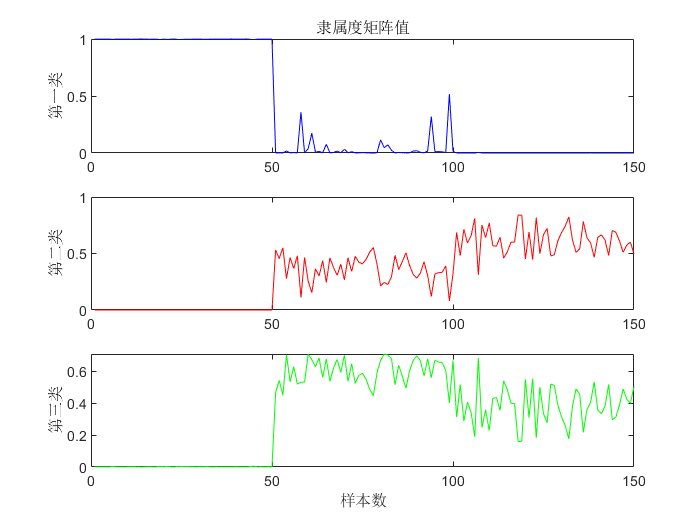
\includegraphics[scale=0.6]{lishudu.png}
    \caption{隶属度矩阵的值}
    \label{隶属度}
\end{figure}
\section{与实际值和FCM算法分类结果比较}
\chapter{总结与展望}
\par 
独立的系统演化是一个熵增的过程,在没有外力的作用下,熵是一直增加的,即符合我们的最大熵原理。
而自然界也是一个巨大的系统,时时刻刻产生信息,有精确的,但许多都是模糊的。
为了在已有的知识下,使我们的结果更加准确,我们趋向于使得信息的熵最大,于是我们在FCM的基础上融入了最大熵模型,形成了模糊最大熵模型。
最后我们将模糊最大熵模型应用于iris数据集的分类,取得了相对于FCM算法更好的聚类效果。
\par
现如今,适逢新一代人工智能的浪潮,各种智能算法、机器学习研究论文层出不穷,而模糊聚类在图像分割、目标识别、故障诊断等方面也有广泛的应用,
相信在不久的未来,关于模糊最大熵模型的应用于机器学习的结合会越来越多,推动模糊分类算法变得越来越好。

%%%%%%%%%%%%%%%%%%%%%%%%%%%%%%
%% 附件部分
%%%%%%%%%%%%%%%%%%%%%%%%%%%%%%
%\backmatter

% 参考文献
% 使用 BibTeX
\phantomsection
\addcontentsline{toc}{chapter}{参考文献}
\bibliography{bib/ahu}
\nocite{*} % for every item

% 致谢
\chapter{致谢}
% 附录
\begin{appendix}
	\include{chapter/code}
\end{appendix}



\end{document}
